\chapter{Sensores e Atuadores}
\label{cap:3}

\section{Considerações Iniciais}
Um sensor é um dispositivo que detecta ou mede um quantitativo físico e o transforma, normalmente, em um sinal
elétrico. O dispositivo oposto é o atuador, que converte um sinal elétrico para alguma ação, normalmente
mecânica \cite{sinclair2001}.

Um transdutor é definido como qualquer dispositivo que converte um tipo de energia para outro. Alguns
autores diferenciam-os de sensores, seja alegando que transdutores possuem uma preocupação maior com a eficiência
da conversão de energia ou que o sensor é apenas uma parte do transdutor responsável por detectar a variável
do ambiente \cite{sinclair2001,kondrasovas2013}.

Contudo, neste trabalho considera-se que, por definição, sensores e atuadores são tipos de transdutores.

\section{Sensores}
Avanços tecnológicos recentes tem permitido o desenvolvimento de dispositivos sensores de baixo custo, baixo
consumo de energia e pequenos portes. Eles podem medir distância, direção, velocidade, umidade, temperatura, luz,
vibração, pressão, propriedades acústicas e muitos outros atributos \cite{hai_nayak_stojmenovic2010}.

De acordo com \citeonline{karl_willig2005}, os sensores podem ser divididos em três categorias:
\begin{itemize}
	\item \textbf{Passivos e omnidirecionais:} medem informações físicas sem manipular o ambiente,
	utilizando apenas os fenômenos existentes (vibração, luz, radiação, etc). Além disso, não possuem
	noção de direção envolvida na medição. A maioria dos sensores pertencem à esta categoria, alguns
	exemplos são sensores de temperatura, luz, umidade, gases, entre outros.
	\item \textbf{Passivos e de feixe estreito:} diferenciam-se dos anteriores pois possuem uma noção bem
	definida de direção. Um exemplo típico é uma câmera.
	\item \textbf{Ativos:} ao contrário dos anteriores, sensores deste tipo emitem algum tipo de sinal,
	como ondas ou elétrons, e captam as informações através do reflexo desses sinais emitidos. Os
	exemplos mais conhecidos são os sensores sonares, radares e sísmicos.
\end{itemize}

Também podem ser classificados quanto à referência selecionada, sendo ela absoluta ou relativa. Um sensor
absoluto converte um estímulo para uma escala física absoluta que é independente das condições de medição, já
um sensor relativo produz um sinal que se refere à algum caso especial. Os sensores de pressão, por exemplo,
podem ser absolutos, cujo sinal produzido é relativo ao vácuo (zero absoluto na escala de pressão), ou
relativos, que poduzem sinais referentes à algum patamar, como a pressão atmosférica \cite{fraden2010}.

Uma maneira lógica de classificá-los é através da propriedade física que está sendo medida, como
temperatura, pressão, movimento, etc \cite{kenny_walt2005}.

Podem também ser divididos em analógicos e digitais. Segundo \citeonline{thomazini_albuquerque2005}, um sensor
analógico é capaz de assumir qualquer valor em seu sinal de saída ao longo do tempo, desde que esteja dentro
da sua faixa de operação, já um digital pode assumir apenas dois valores, que podem ser interpretados como
zero ou um, após serem convertidos pelo circuito eletrônico do transdutor.

Há diversas características relevantes quando se trata de sensores, uma delas é a resolução, que mede a
menor alteração do quantitativo físico que um sensor consegue detectar \cite{sinclair2001}.

Outra característica importante é a área de cobertura ou alcance de um sensor, que consiste na distância em
que ele consegue captar a informação de maneira precisa e confiável \cite{karl_willig2005}.

Além desses, existem alguns outros atributos que caracterizam um sensor, sendo eles: sensibilidade, a relação
entre o sinal físico de entrada e o elétrico de saída; exatidão, a diferença entre o valor real e o valor
gerado pelo sensor; precisão, a capacidade de reproduzir os resultados que foram obtidos experimentalmente da
mesma forma; ruído, produzido pelo sensor a adicionado ao sinal de saída; largura de banda ou tempo de
resposta, velocidade com que o sensor consegue prover uma corrente de leitura
\cite{kenny_walt2005,kondrasovas2013}.

\subsection{Temperatura}
Devido à grande significância de seu efeito em materiais, a temperatura é a variável mais medida e determina o
grau de ``quentura'' ou ``frieza'' referenciada à uma escala específica. Ela é proporcional à taxa de energia
cinética das moléculas e átomos pertencentes a um objeto ou sistema.
\cite{fontes2005,peeters_peetermans_indesteege2007}.

Segundo \citeonline{fontes2005}, sensores de temperatura detectam uma mudança em um parâmetro físico, como
resistência ou tensão de saída, que corresponde à uma mudança de temperatura e que pode ser medida através de
duas maneiras:

\begin{itemize}
	\item \textbf{Com contato:} requer que o sensor esteja em contato físico direto com o objeto ou
	sistema a ser mensurado;
	\item \textbf{Sem contato:} a medição interpreta a energia radiante de uma fonte de calor emitida na
	faixa infravermelha do espectro eletromagnético.
\end{itemize}

Essa leitura pode ser realizada de maneira estática, onde a temperatura do corpo permanece estável, e
dinâmica, quando a temperatura varia durante a medição. No caso da leitura dinâmica, existe um tempo de
retardo entre a temperatura e o valor medido que é chamado de erro dinâmico. Esse erro depende do tempo de
resposta do sensor e da taxa de variação da temperatura \cite{peeters_peetermans_indesteege2007}.

Os sensores de temperatura absoluta utilizam como referência o zero absoluto (0 K) ou qualquer outro ponto na
escala de temperatura absoluta, como o 0ºC (273.15 K), já os relativos medem a diferença de temperatura entre
dois objetos, sendo um deles a referência \cite{fraden2010}.

Existem diversos tipos de sensores de temperatura, cada qual com suas vantagens e desvantagens de acordo com
a aplicação. A seguir serão apresentados quatro dos principais tipos.

\subsubsection{Termorresistências}
Também chamados de RTD (\textit{Resistance Temperature Detector}), são sensores de temperatura cujo
funcionamento se baseia na variação de resistência elétrica do elemento condutor em função da temperatura.
Esse elemento responsável pela medição pode ser platina, níquel ou cobre \cite{thomazini_albuquerque2005}.

A platina possui a relação entre temperatura e resisistência mais estável sobre a maior faixa de temperatura.
Já o cobre possui a resistência mais linear mas oxida facilmente e o níquel é o mais barato porém possui uma
faixa de temperatura limitada \cite{burns2014}.

Devido à essa grande estabildiade e exatidão, a termorresistência mais utilizada é a de platina, sendo capaz de
trabalhar na faixa de -200ºC a 850ºC \cite{thomazini_albuquerque2005}.

A figura \ref{figura:rtd} mostra um modelo de RTD que contém uma cabeça de conexão que é comumente utilizada
neste tipo de sensor e serve para fornecer uma transição entre o RTD e a fiação da aplicação além de prover
uma proteção contra condições ambientais, como água e outros contaminantes \cite{burns2014}.

\begin{figure}[h]
	\caption{RTD com cabeça de conexão}
	\centering
	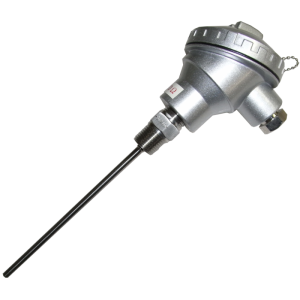
\includegraphics[scale=1.8]{../images/rtd.png}
	\hspace{\linewidth}
	Fonte: http://www.apcs.net.au
	\label{figura:rtd}
\end{figure}

\subsubsection{Termistores}
Assim como os RTDs, os termistores são dispositivos que alteram a resistência elétrica em relação à
temperatura. No entanto, são formados por semicondutores fabricados com misturas de óxidos metálicos
\cite{white_sapoff2014}.

Há dois tipos diferentes de termistores disponíveis: PTC (\textit{Positive Temperature Coefficient}), que
exibem um aumento de resistência ao passo que a temperatua aumenta e NTC (\textit{Negative Temperature
Coefficient}), que decrementam a resistência elétrica de acordo com o crescimento da temperatura
\cite{fontes2005}.

Os termistores do tipo PTC possuem um coeficiente de temperatura extremamente variável, que é denominado por
uma região de temperatura em que o coeficiente de resistência aumenta rapidamente. Fora desse limite, o
coeficiente é negativo ou nulo, o que os torna não viáveis para medições de temperatura
\cite{white_sapoff2014,thomazini_albuquerque2005}.

Os do tipo NTC, por outro lado, são ideais para medições de temperatura, pois mesmo operando com uma faixa de
temperatura útil pequena em comparação à um RTD, por exemplo, conseguem realizar medições mais sensíveis
dentro dessa faixa, que normalmente varia entre -80ºC à 250ºC \cite{sinclair2001,thomazini_albuquerque2005}.

Devido ao simples processo de fabricação, termistores podem ser feitos em escala pequena, conforme ilustrado na
figura \ref{figura:ntc}, o que torna o tempo de resposta térmico extremamente rápido
\cite{peeters_peetermans_indesteege2007,sinclair2001}.

\begin{figure}[h]
	\caption{Modelo de termistor NTC}
	\centering
	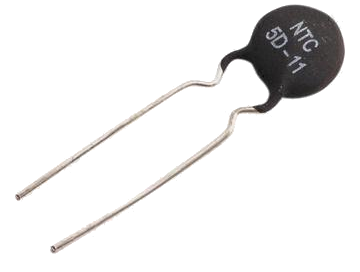
\includegraphics[scale=0.3]{../images/thermistor.png}
	\hspace{\linewidth}
	Fonte: http://www.globalsources.com
	\label{figura:ntc}
\end{figure}

\subsubsection{Termopares}
Também chamados de sensores de contato termoelétrico, os termopares são formados quando dois condutores
elétricos de metais diferentes são ligados à uma extremidade de um circuito. Entretanto, é necessário ter
pelo menos duas ligações para obter um sensor prático. Desse modo, esses sensores possuem uma ligação de
medição, que é exposta à temperatura do processo, e uma ligação de referência, que é mantida à uma referência
de temperatura conhecida \cite{fraden2010,fontes2005}.

Quando as duas junções estiverem em temperaturas diferentes, uma corrente irá fluir pelos fios
proporcionalmente à essa diferença. A temperatura na junção de medição pode então ser determinada a partir do
tipo de termopar utilizado e da temperatura da junção de referência \cite{fraden2010}.

Os termopares, exemplificados pela figura \ref{figura:thermocouple}, são amplamente utilizados em ambientes
industriais, pois são os que cobrem a maior faixa de temperatura (-200 a 2.3000ºC aproximadamente) e possuem
uma boa exatidão e precisão \cite{thomazini_albuquerque2005}.

\begin{figure}[h]
	\caption{Exemplo de termopar}
	\centering
	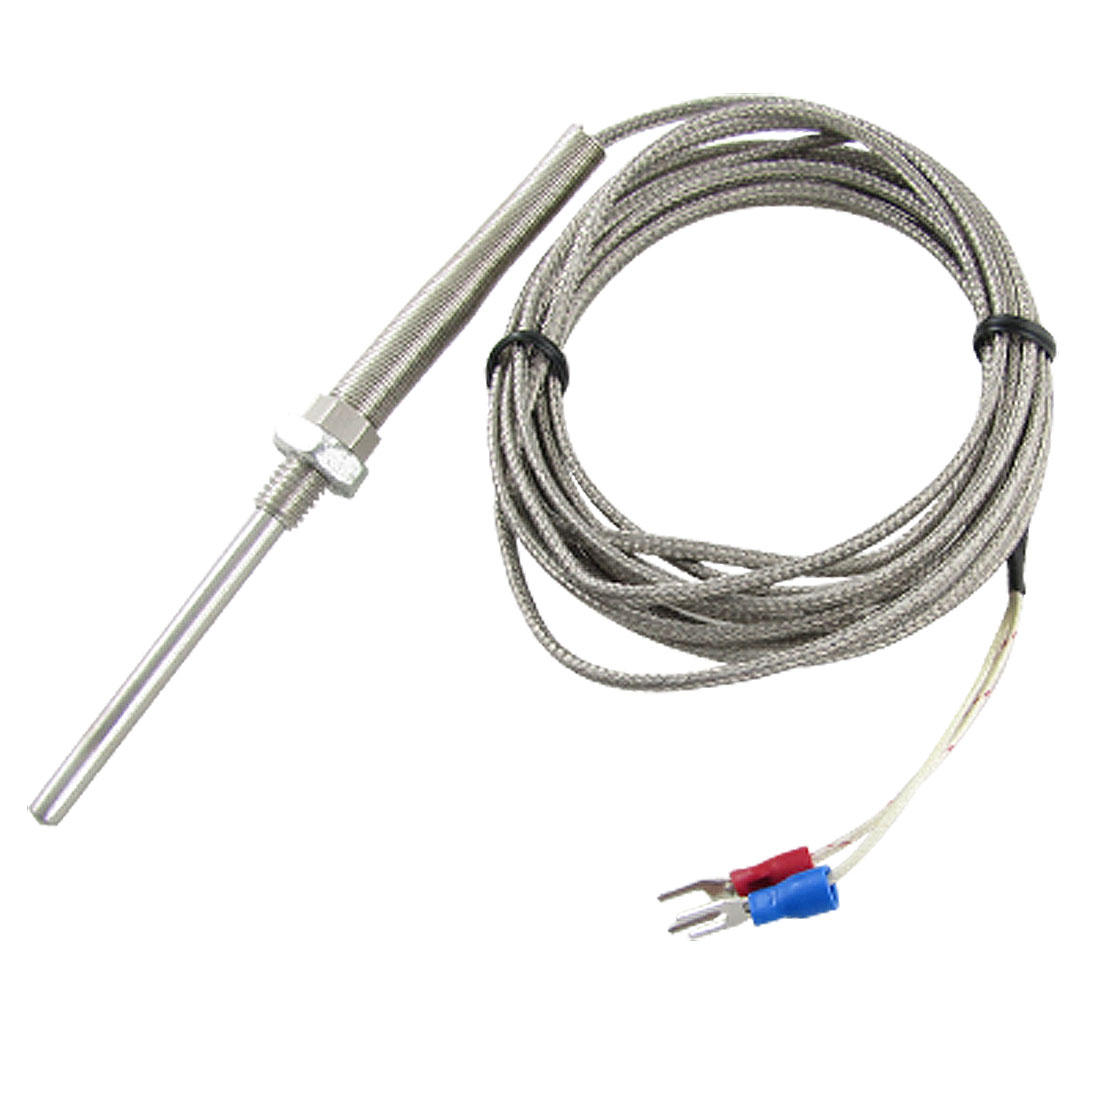
\includegraphics[scale=0.15]{../images/termopar.jpg}
	\hspace{\linewidth}
	Fonte: http://www.kalkaheater.com
	\label{figura:thermocouple}
\end{figure}

\subsubsection{Eletrônicos}
São dispositivos à base de silício que utilizam propriedades de resistência elétrica para medir a temperatura
e oferecem uma curva de resistência quase linear. Dois grandes exemplos são os diodos, que possuem um
decaimento de tensão para cada aumento de grau térmico, e os transistores, cujos parâmetros variam com a
temperatura \cite{thomazini_albuquerque2005}.

Esses sensores eletrônicos também podem vir na forma de circuito integrado, que além de fornecer uma leitura
de temperatura direta e digital, também possuem outras funções como filtros, reguladores e proteções
\cite{fontes2005,thomazini_albuquerque2005}.

A figura \ref{figura:e-thermsensor} mostra um sensor de temperatura eletrônico que utiliza um diodo para
efetuar a medição.

\begin{figure}[h]
	\caption{Sensor de temperatura eletrônico}
	\centering
	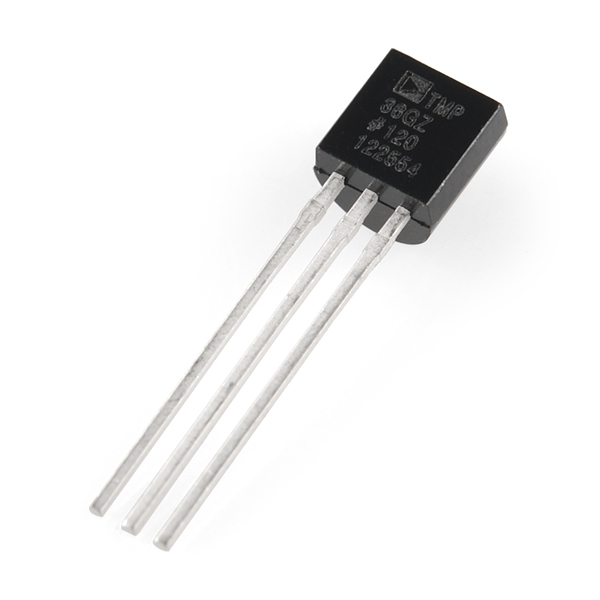
\includegraphics[scale=0.8]{../images/e-thermsensor.jpg}
	\hspace{\linewidth}
	Fonte: https://www.sparkfun.com
	\label{figura:e-thermsensor}
\end{figure}

\subsubsection{Critério de Escolha}
Os quatro tipos apresentados são opções viáveis para medição de temperatura, porém, os que mais se adequam a
aplicações residenciais são os termistores e eletrônicos, pois atuam em uma faixa de temperatura compatível
com a encontrada nesse tipo de ambiente e possuem um ótimo custo-benefício.

Os termopares são os menos estáveis e sensíveis e requerem fios de extensão especiais. Já os RTDs, apesar de
serem os mais exatos e precisos, são relativamente grandes e caros \cite{fontes2005}.

\subsection{Luz}
São considerados sensores de luz dispositivos que são capazaes de detectar radiação eltromagnética na faixa
espectral entre microondas e ultravioleta, que engloba as radiações infravermelhas e a luz visível ao olho
humano. Esses sensores podem ser divididos em quânticos e térmicos \cite{fraden2010}.

A luz e as demais formas de radiação possuem partículas elementares chamadas fótons, que são responsáveis por
quantificar a força eletromagnética. Os sensores quânticos absorvem esses fótons e emitem elétrons contendo a
energia radioativa correspondente, efeito conhecido como fotoelétrico. Já os sensores térmicos, recebem a
radiação infravermelha e utilizam um termômetro para medir o aumento de temperatura do corpo detector
\cite{kenny2005}.

Para aplicações residenciais e prediais, a faixa que mais interessa é a de luz visível. Sendo assim, é
preferível a utilização de sensores de luz quânticos, pois oferecem o melhor desempenho para detecção de
radiação ótica e que geralmente são produzidos nas formas de fotodiodos, fototransistores ou fotoresistores
\cite{fraden2010}.

\subsubsection{Fotodiodos}
O fotodiodo, representado na figura \ref{figura:photodiode}, é um diodo cuja junção de semicondutores está exposta à incidência de raios luminosos, onde a
energia recebida através dos fótons permite com que essa junção se comporte como condutora elétrica
independente da polarização aplicada, gerando assim uma energia elétrica correspondente \cite{sinclair2001}.

\begin{figure}[h]
	\caption{Fotodiodo}
	\centering
	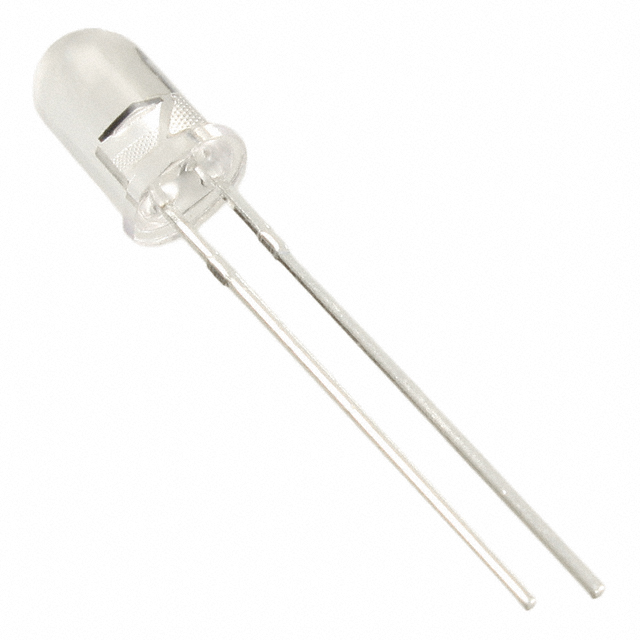
\includegraphics[scale=0.2]{../images/photodiode.jpg}
	\hspace{\linewidth}
	Fonte: http://www.digikey.com
	\label{figura:photodiode}
\end{figure}

Ele possui dois modos de operação, fotovoltaico (FV) e fotocondutivo (FC). No modo FV não há polarização do
diodo, dessa forma, ele opera como um dispositivo gerador de corrente pois converte a energia luminosa em
tensão elétrica. Normalmente é utilizado como uma pequena bateria solar e raramente como sensor \cite{fraden2010}.

Já no modo FC, o diodo é polarizado. Se essa polarização for direta, o aumento de corrente gerado pela
incidência luminosa será pequeno refente à corrente negra (gerada pelo circuito e conduzida pelo diodo na
ausência de luz), tornando-os não muito úteis para atuarem como sensores. Senso assim, normalmente os
fotodiodos no modo FC são inversamente polarizados, gerando uma corrente elétrica quase linearmente
proporcional à intensidade de luz \cite{dado_fischer2007}.

\subsubsection{Fototransistores}
Opera como uma combinação de um fotodiodo polarizado inversamente e um transistor convencional. Dessa forma, a
corrente gerada pelo efeito fotoelétrico na junção do transistor é amplificada, o que torna um fototransistor,
ilustrado na figura \ref{figura:phototransistor},  um sensor de luz extremamente sensível
\cite{dado_fischer2007}.

\begin{figure}[h]
	\caption{Fototransistor}
	\centering
	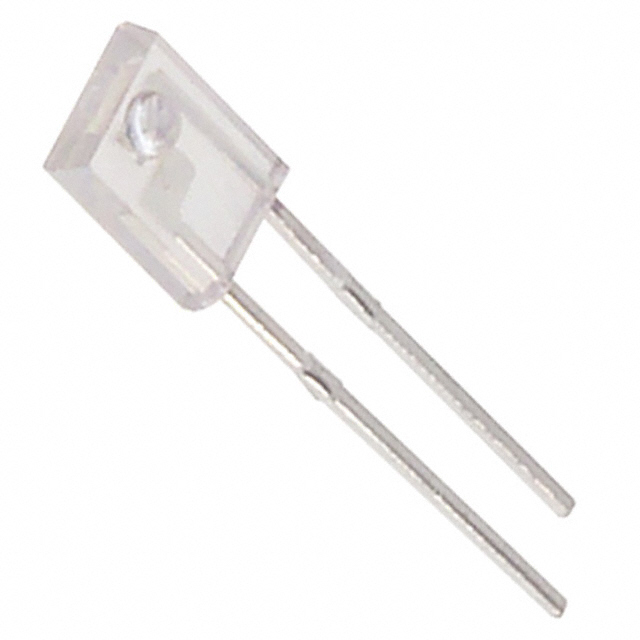
\includegraphics[scale=0.2]{../images/phototransistor.jpg}
	\hspace{\linewidth}
	Fonte: http://www.digikey.com
	\label{figura:phototransistor}
\end{figure}

Contudo, a penalidade para este grande aumento de sensibilidade é um tempo de resposta muito maior que o dos
fotodiodos. Devido a isso, os fototransistores são pouco utilizados, pois é possível obter uma boa
sensibilidade e tempo de resposta utilizando fotodiodos integrados com amplificadores operacionais
\cite{sinclair2001}.

\subsubsection{Fotoresistores}
Também chamados de LDR (\textit{Light Dependent Resistor}), são dispositivos cuja resistência altera sob a
incidência luminosa na superfície, que normalmente é fabricada com materiais baseados em cádmio como o
mostrado na figura \ref{figura:photoresistor}
\cite{dado_fischer2007}.

\begin{figure}[h]
	\caption{Fotoresistor}
	\centering
	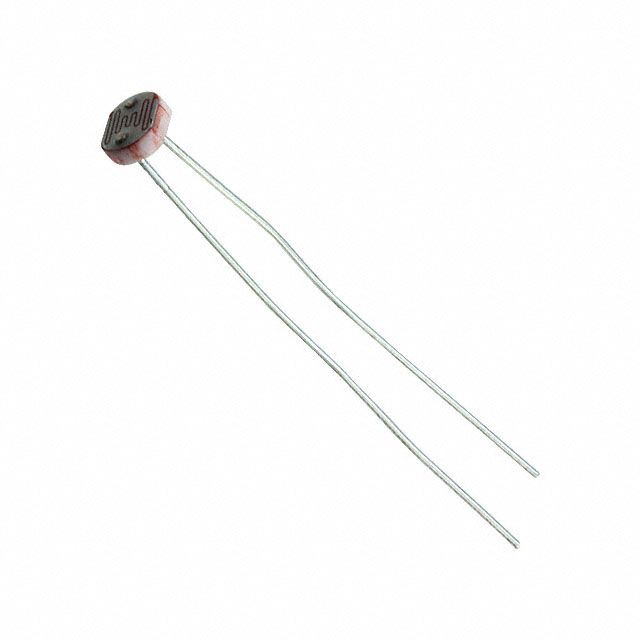
\includegraphics[scale=0.2]{../images/photoresistor.jpg}
	\hspace{\linewidth}
	Fonte: http://www.digikey.com
	\label{figura:photoresistor}
\end{figure}

A sensibilidade desses dispositivos varia dependendo do tamanho da superfície, mas normalmente é maior que a
de um fotodiodo e possuem o pior tempo de resposta entre os três fotosensores mencionados
\cite{thomazini_albuquerque2005}.

\subsubsection{Critério de Escolha}
Embora possuam algumas diferenças de performance, tanto os fotodiodos, fototransisotres e fotoresistores
possuem baixo custo e são opções válidas para atuarem como sensores de luz em uma aplicação residencial.

\subsection{Umidade}
É um quantitativo físico definido como a quantidade de vapor de água contida no ar ou em outros gases e é um
dos fatores mais importantes quando se refere à conforto e bem-estar, juntamente com a temperatura
\cite{fontesII2005,fraden2010}.

A quantidade real de vapor de água, expressa em gramas por metro cúbico de ar (densidade), contida na
atmosfera é chamada de umidade absoluta e muda de acordo com a temperatura do ambiente. Quando o valor máximo
em que essa densidade pode atingitr é alcançado à determinada temperatura, diz-se que o ar está saturado,
condição conhecida como ponto de orvalho. Com isso, é possível obter a chamada umidade relativa, que é o
quociente entre a umidade absoluta e o ponto de orvalho \cite{fraden2010,thomazini_albuquerque2005}.

Os avanços recentes no desenvolvimento de tecnologias semicondutoras permitiram a existência de sensores de
umidade que são altamente precisos, duráveis e eficazes em relação ao custo. Os mais comuns são os
capacitivos, resistivos e termicamente condutivos \cite{fontesII2005}.

\subsubsection{Capacitivos}
São sensores de umidade relativa que respondem às variações de quantidade de vapor de água alterando a
permissividade relativa\footnote{Permissividade relativa é uma propriedade que indica o quão facilmente um
material dielétrico pode se tornar polarizado pela imposição de um campo elétrico sobre ele
\cite{engineeringtoolbox}.} de maneira diremante proporcional. Podem funcionar à altas temperaturas de ambiente
(até 200º C) e representam mais de 75\% dos sensores de umidade disponíveis no mercado
\cite{farahani_wagiran_hamidon2014}.

O modelo mostrado na figura \ref{figura:capacitive_humidity} é um exemplo desse tipo de sensor.

\begin{figure}[h]
	\caption{Sensor de umidade capacitivo}
	\centering
	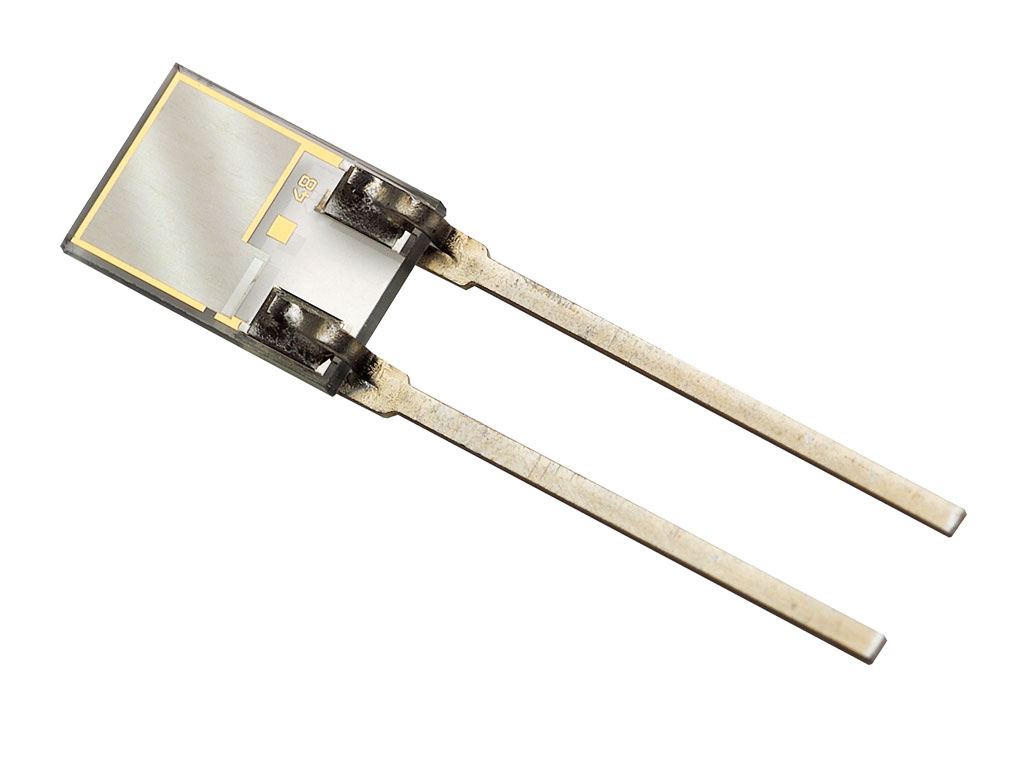
\includegraphics[scale=0.18]{../images/capacitive-humidity.jpg}
	\hspace{\linewidth}
	Fonte: http://www.epluse.com
	\label{figura:capacitive_humidity}
\end{figure}

\subsubsection{Resistivos}
Medem a variação da impedância elétrica\footnote{Impedância elétrica é a medição da oposição que um circuito
possui em relação à corrente elétrica \cite{britannica_2015}.} gerada por um relacionamento exponencialmente
inverso com a umidade \cite{fontesII2005}.

Assim como os capacitivos, também são sensores de umidade relativa, e estão representados pela figura
\ref{figura:resistive_humidity}.

\begin{figure}[h]
	\caption{Sensor de umidade resistivo}
	\centering
	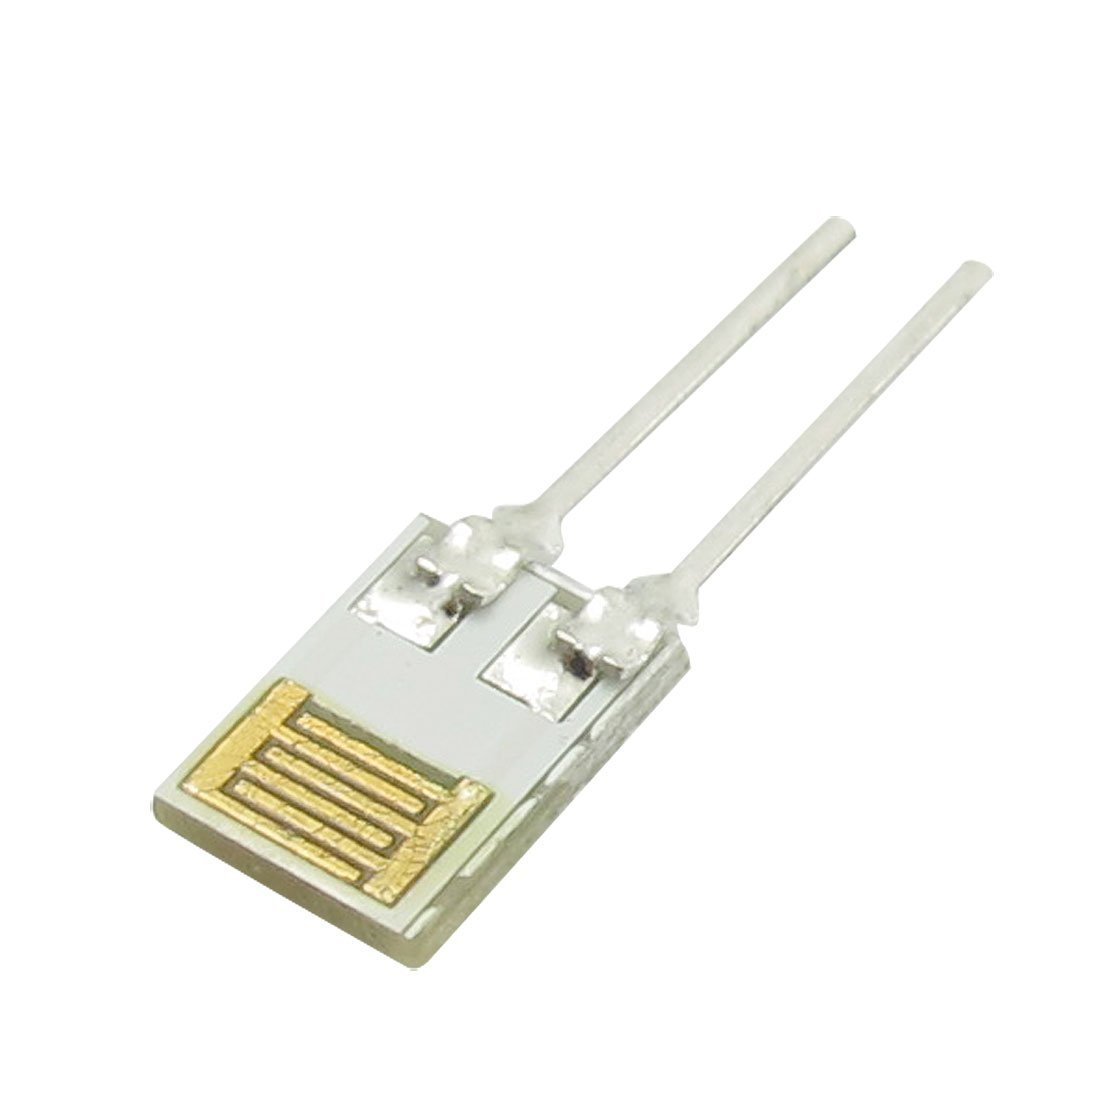
\includegraphics[scale=0.18]{../images/resistive-humidity.jpg}
	\hspace{\linewidth}
	Fonte: http://www.amazon.co.uk
	\label{figura:resistive_humidity}
\end{figure}

\subsubsection{Termicamente Condutivos}
É possível utilizar a condutividade térmica do ar para medir a umidade através de um sensor baseado em
termistor. Esse tipo de sensor utiliza dois termistores NTC conectados por um circuito ponte, onde um deles é
exposto ao gás atmosférico e o outro é hermeticamente selado em ar seco. A diferença das resistências entre os
dois é diretamente proporcional à umidade absoluta \cite{fraden2010,fontesII2005}.

Na figura \ref{figura:thermal_conductivity_humidity} tem-se um sensor termicamente condutivo, sendo que à
esquerda são mostrados os dois termisotres que o compõem.

\begin{figure}[h]
	\caption{Sensor de umidade termicamente condutivo}
	\centering
	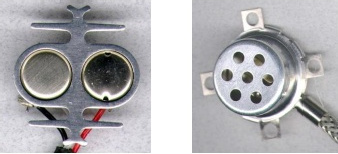
\includegraphics[scale=0.65]{../images/conductivity-humidity.jpg}
	\hspace{\linewidth}
	Fonte: http://www.ohmicinstruments.com
	\label{figura:thermal_conductivity_humidity}
\end{figure}

\subsubsection{Umidade em Sólidos}
Diferente da língua inglesa onde há as palavras \textit{humidity} e \textit{moisture} que, em termos práticos,
siginficam a quantidade de água no ar e em material sólido, respectivamente, em português ambas são traduzidas
para umidade.

A maneira mais simples para detectar a presença de umidade em sólidos de composição aproximadamente fixa é
realizar uma leitura de resistência entre conectores postos à um determinada distância sobre o material, pois
a presença de água no mesmo altera sua condutividade elétrica \cite{sinclair2001,fraden2010}.

Um das utilizaçãoes mais comum deste tipo de detecção é para verificação de umidade em solos, que embora não
resulta em uma medição precisa, é suficiente para determinar se uma planta precisa ser regada ou não, por
exemplo \cite{sinclair2001}.

A figura \ref{figura:soil_moisture} exemplifica um sensor de umidade que utiliza esse conceito de
resistividade do solo.

\begin{figure}[h]
	\caption{Sensor de umidade em solo}
	\centering
	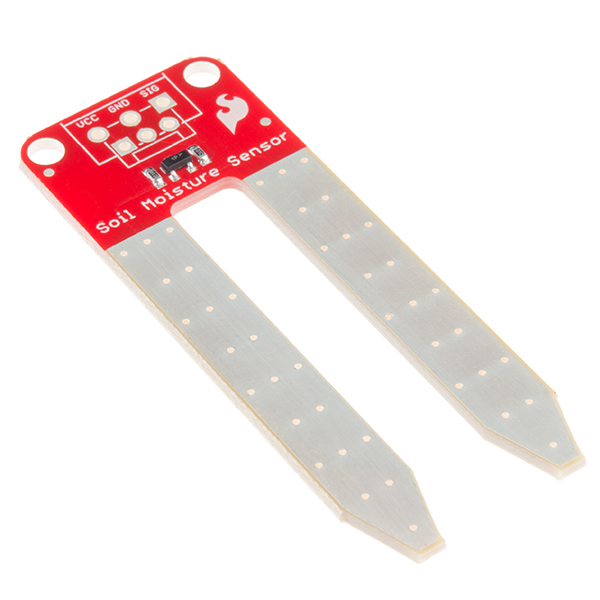
\includegraphics[scale=0.25]{../images/soil_moisture.jpg}
	\hspace{\linewidth}
	Fonte: https://www.sparkfun.com
	\label{figura:soil_moisture}
\end{figure}

\subsubsection{Critério de Escolha}
Realizar a medição de umidade absoluta do ar é uma técnica bastante utilizada em alguns utensílios, como forno
de microondas e secadoras de roupa, e em processos industriais, como máquinas de secagem e desidratação de
alimentos \cite{fontesII2005}.

Contudo, para aplicações residenciais é mais viável e prático medir a umidade relativa do ar, podendo utilizar
tanto os sensores capacitivos quanto os resistivos, além, é claro, de utilizar sensores de umidade em sólidos.

\subsection{Gás e Fumaça}
A detecção de gás é um dos principais fatores quando se trata de segurança, seja em ambientes residenciais ou
industriais, devido a existência de gases tóxicos e inflamáveis, como o monóxido de carbono. Além disso, a
presença desse tipo de gás pode indicar ocorrências de incêndios, juntamente com a detecção de fumaça, que
consiste em um conjunto de fragmentos sólidos, partículas líquidas e gases emitidos normalmente em um
processo de combustão \cite{mulholland1995}.

Em relação aos gases, são utilizados sensores químicos que reagem à determinada composição molecular. Quanto à
fumaça, há os sensores inônicos e ópticos, que são externamente semelhantes conforme mostrado na figura
\ref{figura:smoke}.

\begin{figure}[h]
	\caption{Sensor de fumaça}
	\centering
	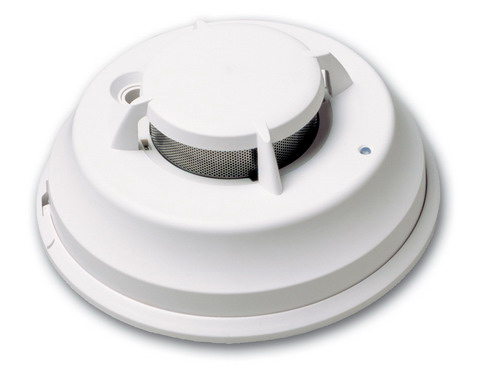
\includegraphics[scale=0.35]{../images/smoke.jpg}
	\hspace{\linewidth}
	Fonte: http://www.dsc.com
	\label{figura:smoke}
\end{figure}

\subsubsection{Químicos}
De acordo com \citeonline{mcmahon2007}, um sensor químico pode ser definido como um dispositivo que possui uma
membrana sensitiva e que gera um sinal em resposta à alguma reação química, como uma ligação entre duas
moléculas.

Duas características importantes para sensores químicos são a seletividade, que descreve o grau em que o sensor
responde apenas para o composto desejado, e a sensibilidade ao composto alvo, que dita a concentração mínima
necessária para que determinado alvo seja detectado \cite{fraden2010}.

A figura \ref{figura:gas} contém um sensor de monóxido de carbono que gera uma resistência como sinal de
saída de acordo com a concentração do gás.

\begin{figure}[h]
	\caption{Sensor de gás}
	\centering
	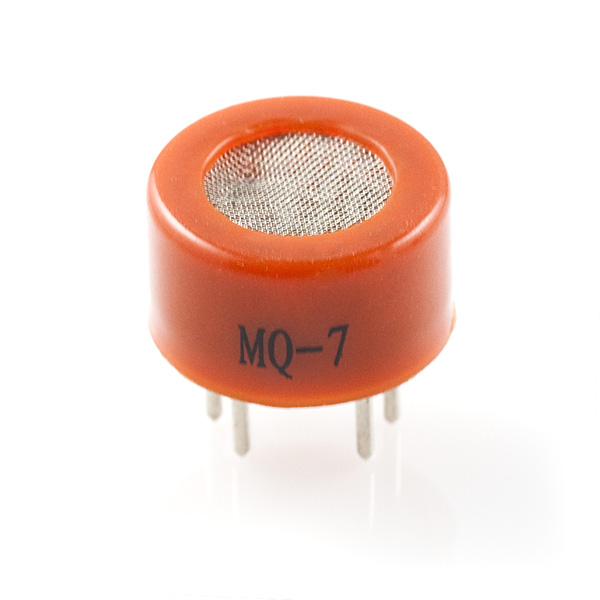
\includegraphics[scale=0.5]{../images/carbon-monoxide.jpg}
	\hspace{\linewidth}
	Fonte: https://www.sparkfun.com
	\label{figura:gas}
\end{figure}

\subsubsection{Iônicos}
Consiste de uma fonte fraca de material radioativo entre duas superfícies metálicas com uma diferença de
pontencial entre elas, tudo dentro de um espaço chamado câmara de ionização\footnote{Ionização é a geração de
partículas eletricamente positivas ou negativas.}. As partículas provenientes desse material ionizam o ar
contido nesse espaço o que permite uma pequena corrente elétrica passar entre os dois eletrodos.  Desse modo,
as partículas de fumaça, ao entrarem na câmara de ionização farão com que essa corrente diminíua, ativando
assim o sensor \cite{sinclair2001}.

\subsubsection{Ópticos}
Baseiam-se no uso de um LED pulsante e de uma célula fotoelétrica posicionada de forma a não receber nenhum
tipo de luz. No momento em que ocorre a entrada de fumaça nesse ambiente, a mesma dispersa os raios luminosos do
LED que refletem sobre o sensor fotoelétrico \cite{thomazini_albuquerque2005}.

\subsubsection{Critério de Escolha}
Em relação aos gases, normalmente utiliza-se sensores de monóxido de carbono e de alguns gases inflamáveis como
metano ou butano.

Quanto aos sensores de fumaça, os iônicos são mais adequados para detectar fogos no estágio de fumaça visível
enquanto os ópticos detectam melhor fogos no estágio latente. Recomenda-se utilizar os dois tipos de sensores
em conjunto \cite{sinclair2001}.

% \section{Atuadores}
